\chapter{动力学分析及建立控制模型}

\section{引言}
本章主要探究影响系统状态的因素,分析这些影响因素的作用模型,
在考虑库伦摩擦力和粘滞摩擦力的接触模型的基础上,推导系统动力学方程。
根据动力学方程分析系统控制的难点,并建立控制模型。

\section{动力学分析及建模}

在实际运动过程中,摩擦情况是十分复杂的。
一般情况下库伦摩擦力和粘滞摩擦力可以较好地体现接触模型中的摩擦特征。
因此本课题中也只考虑库伦摩擦力和粘滞摩擦力。
本课题研究的平行指夹具仅有一个自由度,该夹具让物体在重力作用下竖直下落,
通过控制夹爪之间的距离改变夹持力,从而控制物体停止的位置,如图 2-1 所示。
假设在受控滑动过程中物体能竖直下落,不会因为重心的偏移而发生转动。
在这一假设条件下,记物体顶端到夹具中心点的垂直距离为$h(t)$,
用 $h(t)$ 可以描述任意时刻物体的位置。
本课题的研究目的是改变物体的位置从 ${h_{\rm 0}}({t_{\rm 0}})$ 到一个指定的点 ${h_{\rm d}}({t_{\rm f}})$。
假设机械臂是静止的,我们只控制平行夹爪的张合宽度 $d$ 来改变施加在物体上的夹持力,
从而控制夹爪和物体之间的摩擦力。假设物体在 $t$ 时刻的状态 $x(t) = {\left[ {h(t),\dot h(t)} \right]^{\rm T}}$ 可以通过传感器测量。

\begin{figure}[!ht]
  \centering
  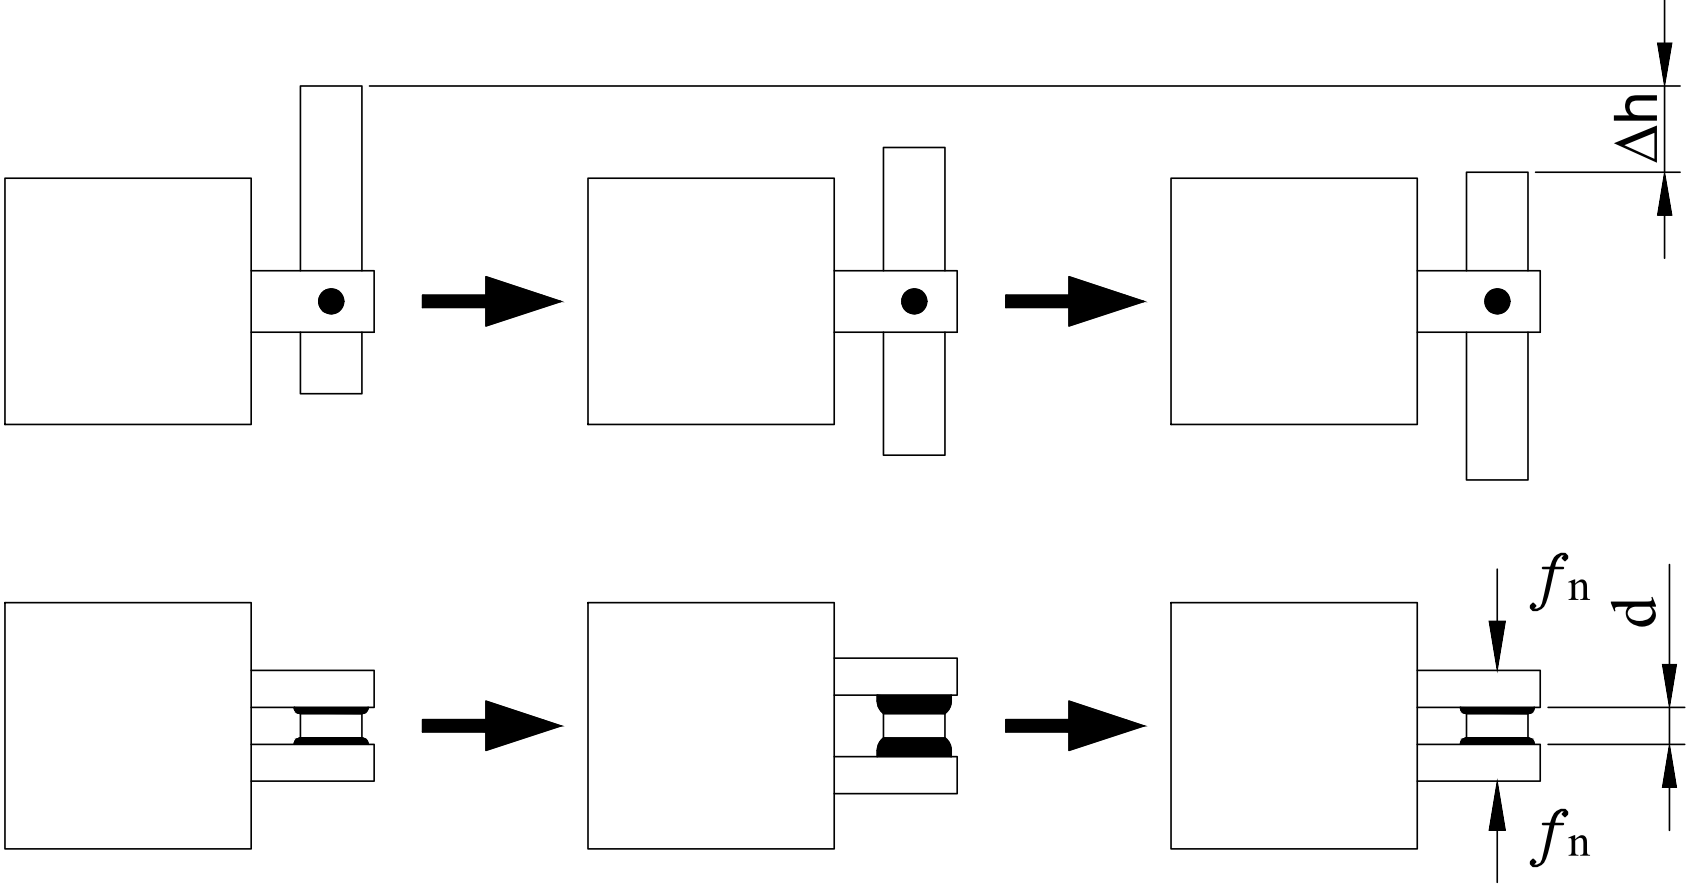
\includegraphics[width=13cm]{chapter02/pic/2-1}
  \caption{通过重力和受控滑动实现工具的在手操作}
  \label{fig:2-1}
  \vspace{-0.3cm}
\end{figure}

该项目中通过夹具和工具接触产生的滑动摩擦力控制工具运动,由于忽略工具的转动,
因此工具的滑动摩擦力可近似用库伦摩擦力和粘滞摩擦力表示 \cite{ref9}。即

\begin{equation}
  f({f_{\rm n}},\dot h) =  - \mu {\mathop{\rm sgn}} (\dot h){f_{\rm n}} - \sigma \dot h
  \label{equ:2-1}
\end{equation}

\begin{note}
  \para{$\mu$}{夹具与物体接触表面之间的滑动摩擦系数;}
  \para{${f_{\rm n}}$}{指尖施加在物体表面的正压力${\rm{(N)}}$;}
  \para{$\dot h$}{物体下降速度$\rm(m/s)$;${\mathop{\rm sgn}} ( \cdot )$为符号函数;}
  \para{$\sigma$}{粘滞摩擦系数$\rm(N\cdot s/m)$。}
\end{note}

从式\ref{equ:2-1}中可以得到正压力和摩擦力之间的关系。
因此通过压力传感器测量出夹具施加给工具的法向力后,
我们就能定量估计工具受到的摩擦力。

该系统的动力学模型为单自由度的直线受控滑动,其动力学方程用牛顿第二定律可以表示为
\begin{equation}
  m\ddot h =  - mg + f
  \label{equ:2-2}
\end{equation}

\begin{note}
  \para{$m$}{物体质量$\rm(kg)$;}
  \para{$g$}{重力加速度$\rm(m/s^2)$;}
  \para{$f$}{夹爪和物体接触产生的摩擦力$\rm(N)$。}
\end{note}

% \noindent 式中$m$为工具质量$(kg)$, $g$ 是当地重力加速度$(m/s^2)$, $f$ 为夹爪和工具接触产生的摩擦力$(N)$。
将摩擦力模型(式\ref{equ:2-1})带入式(\ref{equ:2-2})得到该系统的动力学方程如下

\begin{equation}
  m\ddot h =  - mg + \mu {f_{\rm n}} - \sigma \dot h
  \label{equ:2-3}
\end{equation}


\section{设计控制算法}
参照标准自适应控制模型,根据系统动力学方程推导系统的控制方程,
建立该系统的自适应控制模型。以夹具位移信号为控制量,
实现让工具沿期望的轨迹下落到指定位置。

模型参考自适应控制系统属于自适应控制系统的一种。
它通过设计适应性机构使被控对象和已知参考模型的动态特性趋于一致。
它的原理是基于系统的输出信号与期望信号之间的误差实时地修正系统的结构参数,
从而实现系统输出信号与参考模型的输出信号的误差收敛到零。
自适应控制模型的构成如图 \ref{fig:2-2} 所示,可分为四部分:
含有未知参数的被控对象、提供系统理想输出的参考模型、包含可调节参数的反馈控制定律,
以及修正可调参数的控制器 \cite{ref10} 。
该控制系统的特性要求,如超调量、阻尼性能、过渡时间和通频带等由参考模型规定,
故参考模型实际上是被控对象的理想输出模型,其输出代表了期望的性能。
当实际被控对象与参考模型输出有差异时,
控制器会通过自适应机构改变控制器参数或生成辅助输入以消除误差,
使实际输出量和参考模型输出一致。

\begin{figure}[!ht]
  \centering
  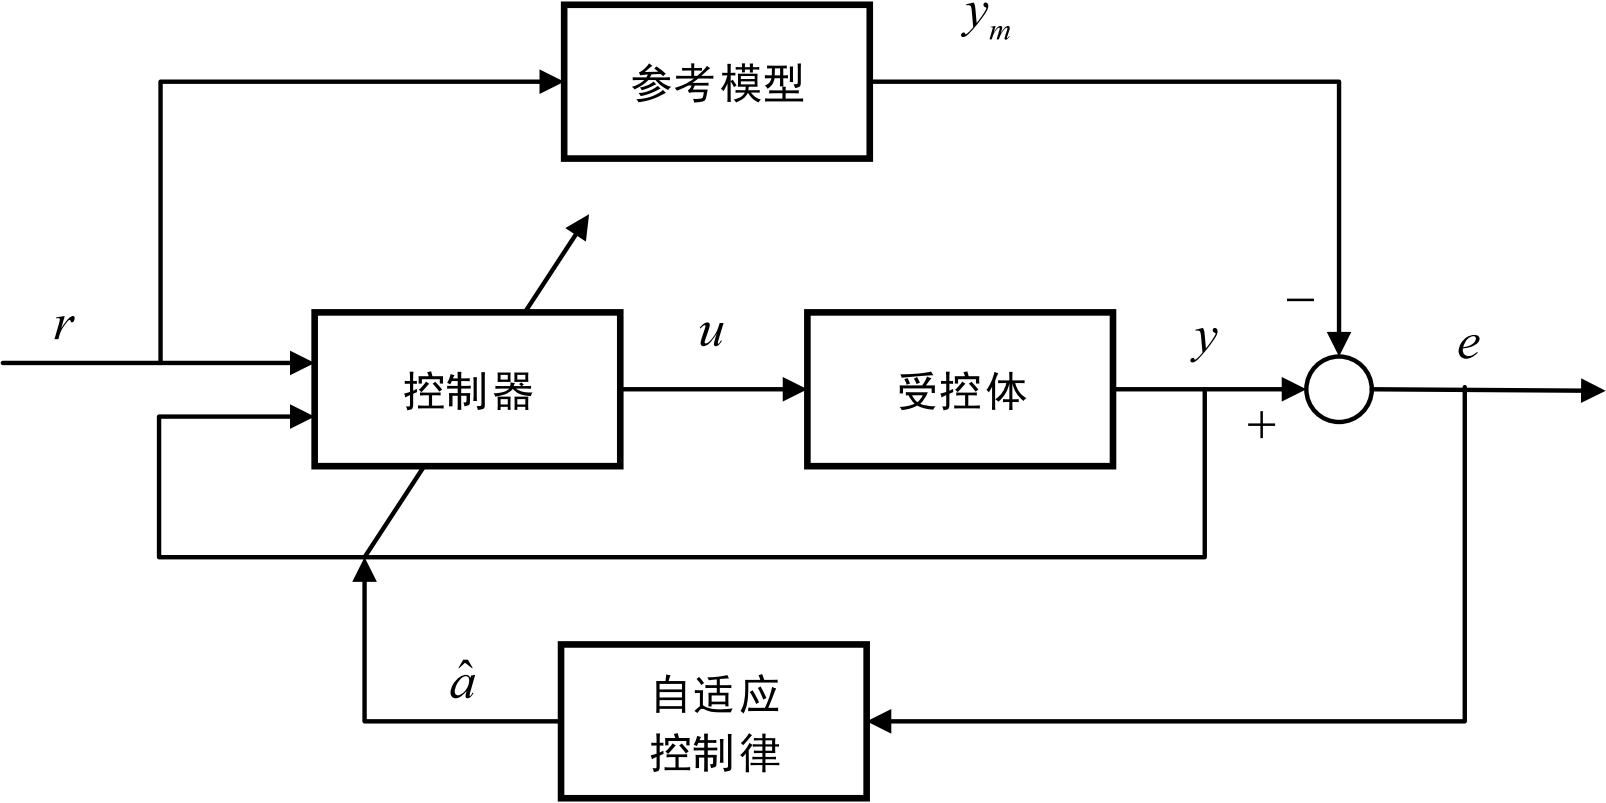
\includegraphics[width=12cm]{chapter02/pic/2-2}
  \caption{模型参考自适应控制系统简图}
  \label{fig:2-2}
  \vspace{-0.3cm}
\end{figure}

在已知摩擦模型的基础上,要实现对物体间相对运动的控制,接触物体间的摩擦系数也必须给出。
但是测量物体的摩擦系数存在一定的困难,因为它和接触的几何特征及压力分布等有关,
而且不同物体间的摩擦系数不同。这就导致了摩擦模型在实际运用时十分繁琐,应用范围有限。
自适应控制模型正好可以轻易地解决这一难题,它让我们在即便摩擦系数未知,
甚至是物体重量的情况下,也能控制系统输出。也就是说,我们不再需要测量摩擦系数,
而且不用调整系统参数也能实现不同重量的物体的在手操作。

由于该项目需要实现的是被动在手操作,即在重力作用下进行的操作,
所以在我们的位置控制模型中不应该出现超调的情况,
因此我们可以设计一个二阶临界阻尼系统在阶跃信号下的输出为参考模型。
该参考模型的传递函数为
\begin{equation}
  {G_m}(p) = \frac{{{h_{\rm d}}}}{{{t_{\rm in}}}} = \frac{{\lambda _{\rm 0}^{\rm 2}}}{{{{\left( {p + {\lambda _{\rm 0}}} \right)}^{\rm 2}}}}
  \label{equ:2-4}
\end{equation}

\begin{note}
  \para{$t_{\rm in}$}{系统输入信号$\rm (s)$;}
  \para{$h_{\rm d}$}{系统参考模型的输出信号$\rm(m)$;}
  \para{$\lambda _{\rm 0}$}{控制常量;}
  \para{$p$}{Laplace变量。}
\end{note}

% 式中$h_{in}$,$h_d$分别为系统的输入信号和参考输出;${\lambda _0}$为常数;
% $p$为Laplace变量。

为了建立自适应控制模型,将正压力视为控制系统的输入 $u_{f_{\rm n}}$ ,
将式(2-3)写为控制模型的标准形式如下
\begin{equation}
  a\ddot h + b\dot h + cg = {u_{{f_{\rm n}}}}
  \label{euq:2-5}
\end{equation}
式中$a = c = {m \mathord{\left/
{\vphantom {m \mu }} \right.
\kern-\nulldelimiterspace} \mu }$ , $b = \sigma /\mu $。
记控制系统的跟踪误差为 $s$ ,
\begin{equation}
  s = \dot{\tilde h}  + \lambda \tilde h
  \label{euq:2-6}
\end{equation}

\begin{note}
  \para{$\tilde h$}{物体运动的位置误差$\rm(m)$,$\tilde h = h - {h_{\rm m}}$;}
  \para{$\dot{\tilde h}$}{物体运动的速度误差$\rm(m/s)$,$\dot{\tilde h} = \dot h - {\dot h_{\rm m}}$;}
  \para{$\lambda$}{控制常量$\rm (s^{\rm -1})$,决定广义误差中位置误差的权重。}
\end{note}

% 式中$\tilde h = h - {h_m}$, $\dot{\tilde h} = \dot h - {\dot h_m}$
% 分别表示工具运动的位置和速度误差, $\lambda$ 为一个常数,决定广义误差中位置误差的权重。

进一步,建立标准适应性控制方程 \cite{ref10}
\begin{equation}
  {u_{{f_{\rm n}}}} = \hat a{\ddot h_{\rm r}} - ks + \hat b\dot h + \hat cg
  \label{equ:2-7}
\end{equation}

\begin{note}
  \para{$\ddot h_{\rm r}$}{广义加速度误差$\rm (m/s^{\rm 2})$,${\ddot h_{\rm r}} = {\ddot h_{\rm d}} - \lambda \dot h$;}
  \para{$k$}{跟踪控制增益,为正值。}
\end{note}

该控制方程主要有四部分组成,
前馈加速度项$\hat b{\ddot h_{\rm r}}$, 跟踪误差项$ks$,
速度误差项$\hat b\dot h$, 以及重力补偿项$\hat bg$。
%其中广义加速度误差${\ddot h_r} = {\ddot h_d} - \lambda \dot h$,
%$k$是一个正的跟踪控制增益, 
$\hat a$, $\hat b$, $\hat c$ 分别为可调参数$a$,$b$,$c$ 的估计值, 调参规律如下:
\begin{equation}
  \label{equ:2-8}
  \begin{array}{l}
    \dot{\hat a} = - {\alpha _a}s{{\ddot h}_r}\\
    \dot{\hat b} = - {\alpha _b}s\dot h\\
    \dot{\hat c} = - {\alpha _c}sg
  \end{array}
\end{equation}
式中${\alpha _a}$, ${\alpha _b}$, ${\alpha _c}$ 均为正的自适应增益。
值得注意的是式(\ref{equ:2-8})并不能保证对应的系统结构参数收敛到真值,
但是能保证跟踪误差 $s$ 的收敛,也就意味着能实现物体下落距离的控制。


\section{本章小结}
分析了运动过程中,影响物体相对于机器人手的运动状态的因素,
假定了摩擦模型,进一步建立了系统的运动学方程。
确定了以物体所受正压力为输入,物体运动状态为输出的控制方案。
根据系统动力学方程建立了自适应控制方程,分析了使用该控制算法的合理性。

